% !TeX root = main.tex

\subsection{Anillo de polinomios}

\begin{definition}[Anillo de polinomios]
	Dado un cuerpo $K$, se define el anillo de polinomios en una indeterminada $x$ sobre $K$, denotado $K[x]$, como el conjunto de todas las expresiones formales de la forma
	$$P(x) = a_0 + a_1x + a_2x^2 + \ldots + a_mx^m = \sum_{i=0}^{m} a_i x^i,$$
	donde $n \in \mathbb{N}$ y $a_0, a_1, a_2, \ldots, a_m \in K$. Llamamos grado de $P$, notado $\deg P$, al mayor $k \in \mathbb{N}$ tal que $a_k \neq 0$. Las operaciones de este anillo se definen como:
	\begin{itemize}
		\item Suma ($+$): $$\left(\sum_{i=0}^{m} a_i x^i\right) + \left(\sum_{i=0}^{n} b_i x^i\right) = \sum_{i=0}^{\max\{m,n\}} (a_i + b_i) x^i,$$
		donde se toma $a_i = 0$ o $b_i = 0$ si el índice es mayor que el grado correspondiente.
		\item Producto ($\cdot$): $$\left(\sum_{i=0}^{m} a_i x^i\right) + \left(\sum_{i=0}^{n} b_i x^i\right) = \sum_{k=0}^{m+n}\left(\sum_{i+j=k}a_ib_j\right)x^k.$$
	\end{itemize}
	
	Con estas operaciones, $K[x]$ es un anillo conmutativo cuyo neutro aditivo es $C(x) = 0$ (el polinomio nulo), y cuyo neutro multiplicativo es $I(x) = x$.
\end{definition}

Se observan las siguientes propiedades para el grado de un polinomio:

\begin{itemize}
	\item El polinomio nulo no tiene un grado definido.
	\item $\deg(P + Q) \leq \max\{\deg P, \deg Q\}$.
	\item $\deg(P \cdot Q) = \deg P + \deg Q$.
\end{itemize}

\begin{definition}[Raíz de un polinomio]
	Dados un polinomio $P \in K[x]$ y un $x^* \in \mathbb{K}$, decimos que $x^*$ es una raíz de $P$ si $P(x^*) = 0$.
\end{definition}

Las siguientes propiedades sobre polinomios serán útiles para trabajar con polinomios en las secciones posteriores.

\begin{theorem}[Algoritmo de división de polinomios]
	Sea $K$ un cuerpo y sean $P, Q \in K[x]$ tales que $Q \neq 0$. Entonces, existen únicos polinomios $C, R \in K[x]$ (cociente, resto) tales que $P = Q \cdot C + R$, donde o bien $R = 0$, o bien $\deg R < \deg Q$. 
\end{theorem}

Como corolario de este teorema, se observa que si $x^*$ es una raíz de $P$, entonces al dividir $P$ por el polinomio $x - x*$, se obtiene como resto el polinomio nulo, y vale $\deg Q = \deg P - 1$. Puede ocurrir que $x^*$ sea raíz de $Q$, así como no. Lo que es seguro es que el multiconjunto de raíces de $Q$ (conjunto de raíces contando multiplicidad) se obtiene al quitarle un $x^*$ al multiconjunto de raíces de $P$.

Se observa que se puede interpretar isomórficamente a polinomios como funciones $P: K \to K$. En general, nosotros vamos a trabajar sobre el anillo $\mathbb{F}_p[x]$.

\subsection{Lema de Schwartz-Zippel}

El lema de Schwartz–Zippel es una herramienta fundamental en el estudio de las Pruebas de Identidad de Polinomios (Polynomial Identity Testing, PIT). Las PIT son centrales en los proving systems modernos y aparecen de manera recurrentemente en diversos protocolos criptográficos, donde permiten obtener garantías de corrección probabilísticas.

\begin{theorem}
	Sea $p \in \mathbb{N}$ primo, y sean $P, Q \in \mathbb{F}_p[x]$ dos polinomios de grado a lo sumo $n$. Se toma un $k \in \mathbb{F}_p$ de forma uniformemente aleatoria. Si $P \neq Q$, entonces
	$$\mathbb{P}[P(k) = Q(k)] \leq \frac{n}{p}.$$
\end{theorem}

Para entender intuitivamente este resultado, observemos que como $P, Q$ tienen a lo sumo grado $n$, entonces tienen a lo sumo $n$ raíces cada uno. Es decir que $P(k) = Q(k)$ puede ser verdadero a lo sumo para $n$ valores de entre los $p$ posibles valores de $k$.

En contextos donde el tamaño del cuerpo es significativamente mayor al grado de los polinomios, esta probabilidad resulta despreciable. Por ejemplo, si $p \approx 2^{255}$ y $n = 2^{64}$, entonces $\frac{n}{p} \approx 2^{-191}$. Esto quiere decir que si $P(k) = Q(k)$, es extremadamente probable que $P = Q$. Esto se logra evaluando los polinomios únicamente en un punto, lo que es eficiente.

La hipótesis de elegir $k$ de forma aleatoria es extremadamente importante para la seguridad de los protocolos criptográficos que usan este lema como una de sus herramientas. Si el punto de evaluación pudiera ser elegido de forma maliciosa por un agente que conoce $P, Q$, el lema dejaría de ser aplicable. Ya que si existe un $k^* \in \mathbb{F}_p$ tal que $P(k^*) = Q(k^*)$, entonces el agente malicioso puede usarlo para darnos una garantía (falsa) de que $P = Q$. Esto indica que se requieren mecanismos seguros para la generación de aleatoriedad y su correcta incorporación en los procesos criptográficos que usen el lema de Schwartz-Zippel.

\subsection{Interpolación de polinomios}

\begin{definition}[Polinomio interpolador]
	Sean $K$ un cuerpo, $P \in K[x]$ un polinomio, y $D = \left\{(x_0, y_0), (x_1, y_1), \ldots, (x_n, y_n)\right\}$ un conjunto de puntos de $K \times K$ donde los $x_i$ son distintos dos a dos. Si se cumple $P(x_i) = y_i$ para cada $0 \leq i \leq n$, entonces decimos que $P$ es un polinomio interpolador de $D$.
\end{definition}

\begin{figure}[h]
	\centering
	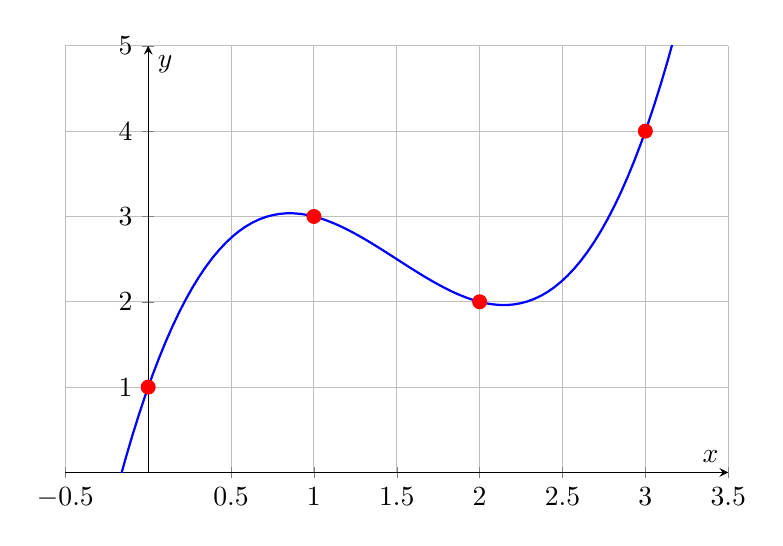
\begin{tikzpicture}
		\begin{axis}[
			axis lines = middle,
			xlabel = $x$,
			ylabel = $y$,
			xmin = -0.5, xmax = 3.5,
			ymin = 0, ymax = 5,
			grid = both,
			width = 10cm,
			height = 7cm,
			samples = 100,
			domain = -0.5:3.5,
			]
			
			% Polinomio interpolador
			\addplot[blue, thick] {x^3 - 9/2*x^2 + 11/2*x + 1};
			
			% Puntos originales
			\addplot[only marks, mark=*, mark size=2.5pt, red] coordinates {
				(0,1) (1,3) (2,2) (3,4)
			};
		\end{axis}
	\end{tikzpicture}
	\caption{Polinomio $P(x) = x^3 - \frac{9}{2}x^2 + \frac{11}{2}x + 1 \in \mathbb{R}[x]$ pasando por $D = \left\{(0,1),(1,3),(2,2),(3,4)\right\}$.}
	\label{fig:interpolacion-polinomio}
\end{figure}


\begin{theorem}[Existencia y unicidad del polinomio interpolador]
	Existe un único polinomio interpolador $P^*$ con $\deg P^* = n$ para un conjunto $D$ de $n$ puntos, y está dado por:
	$$P^*(x) = \sum_{j=0}^{n} y_j L_j(x), \quad L_j(x) = \prod_{i=0, i \neq j}^{n} \frac{x - x_i}{x_j - x_i}.$$
\end{theorem}

Intuitivamente, podemos ver que $L_j(x) = 0$ para cada $i \neq j$, y $L_j(x) = 1$. Así mismo, la unicidad se puede deducir: si hubiera dos polinomios $P, Q$ de grado $n$ que interpolan a un conjunto de $n$ puntos, entonces el polinomio $P - Q$ tendría raíces en $x_0, \ldots, x_n$, lo que son al menos $n + 1$ raíces, contadas con multiplicidad. Esto quiere decir que $P - Q$ es el polinomio nulo, i.e., $P = Q$.

Será muy útil para nosotros calcular el polinomio interpolador en $\mathbb{F}_p[x]$.
